\subsection{Qualità di processo - Documentazione}

\vspace{0.3cm}

\subsubsection{Errori Ortografici}

\vspace{0.3cm}

\begin{figure}[H]
    \centering
    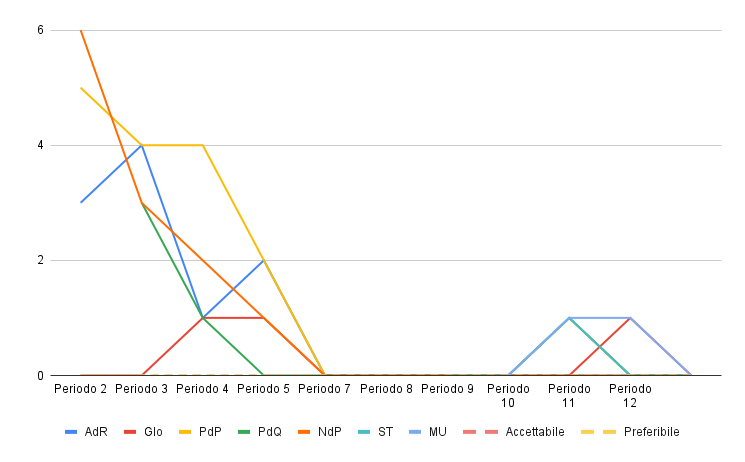
\includegraphics[width=1\textwidth]{../Images/PianoDiQualifica/errori_ortografici.png}
    \caption{Resoconto errori ortografici}
    \label{fig:Errori ortografici}
\end{figure}

\vspace{0.2cm}

\textbf{RTB}: Il grafico mostra l'andamento degli errori ortografici rilevati nei documenti. Si nota come il numero di errori ortografici sia inizialmente alto, ma tenda a diminuire con l'avanzare del progetto.

\vspace{0.2cm}

Questo è dovuto al fatto che il gruppo ha iniziato a prestare maggiore attenzione alla scrittura dei documenti raggiugendo l'ottimo nell'ultimo periodo.

\subsubsection{Indice di Gulpease}

\vspace{0.3cm}

\begin{figure}[H]
    \centering
    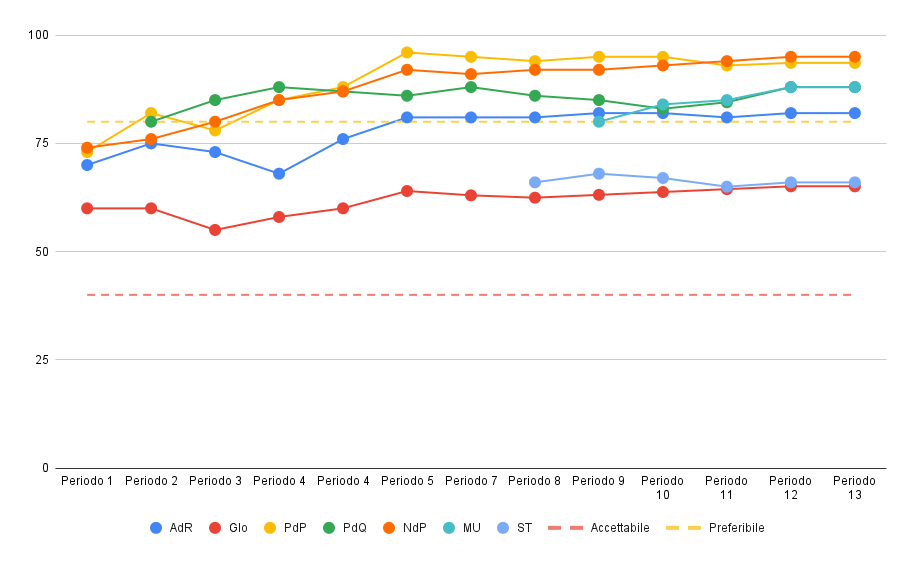
\includegraphics[width=1\textwidth]{../Images/PianoDiQualifica/Gulpease.png}
    \caption{Resoconto indice di Gulpease}
    \label{fig:Indice di Gulpease}
\end{figure}

\vspace{0.2cm}

\textbf{RTB}: Dalla valutazione del grafico si nota un tendenza generale di crescita e/o mantenimento dell'indice per ogni documento durante i vari periodi considerati.

\vspace{0.2cm}

Si osserva che il glossario presenta un indice di Gulpease molto basso, il che è attribuibile alla sua natura tecnica e alla conseguente impossibilità di aumentare tale indice.

\vspace{0.2cm}

Gli altri documenti, invece, mostrano un indice di Gulpease elevato, in parte dovuto al loro contenuto meno tecnico e più accessibile.